% Autor: Alfredo Sánchez Alberca (asalber@ceu.es)

\newproblem{par-1}{gen}{}
%STATEMENT
{Compute the following partial derivatives:
\begin{multicols}{2}
\begin{enumerate}
\item $\dfrac{\partial}{\partial x}\ln \dfrac{x}{y}$.
\item $\dfrac{\partial}{\partial v}\dfrac{nRT}{v}$.
\end{enumerate}
\end{multicols}
}
%SOLUTION
{\begin{enumerate}
\item $\frac{\partial}{\partial x}\,\log \left(\frac{x}{y}\right) = \frac{1}{x}$.
\item $\frac{\partial}{\partial v}\,\left(\frac{n\,R\,T}{v}\right) = -\frac{n\,R\,T}{v^2}$.
\end{enumerate}
}
%RESOLUTION
{
}


\newproblem{par-2}{gen}{}
%STATEMENT
{Compute the gradient vector and Hessian matrix of the following two functions:
\begin{multicols}{2}
\begin{enumerate}
\item $e^{x^2+y^2+z^2}$
\item $\sin((x^2-y^2)z)$
\end{enumerate}
\end{multicols}
}
%SOLUTION
{\begin{enumerate}
\item $\nabla e^{x^2+y^2+z^2} = \left( 2\,x\,e^{z^2+y^2+x^2} , 2\,y\,e^{z^2+y^2+x^2} , 2\,z\,e^{z^2 +y^2+x^2} \right)$,\\
$
H e^{x^2+y^2+z^2} =
\left(
\begin{array}{ccc}
(4x^2+2)e^{x^2+y^2+z^2} & 4xye^{x^2+y^2+z^2} & 4xze^{x^2+y^2+z^2} \\
4xye^{x^2+y^2+z^2} & (4y^2+2)e^{x^2+y^2+z^2} & 4yze^{x^2+y^2+z^2} \\
4xze^{x^2+y^2+z^2} & 4yze^{x^2+y^2+z^2} & (4z^2+2)e^{x^2+y^2+z^2}
\end{array}
\right).
$
\item $\nabla \sen((x^2-y^2)z) = \left( 2\,x\,z\,\cos \left(\left(x^2-y^2\right)\,z\right) , -2\,y\, z\,\cos \left(\left(x^2-y^2\right)\,z\right) , \left(x^2-y^2\right) \,\cos \left(\left(x^2-y^2\right)\,z\right) \right) $\\
$H \sen((x^2-y^2)z) =$\\
\resizebox{\linewidth}{!}{
$
\left(
\begin{array}{ccc}
4x^2\sen((x^2-y^2)z)+2\cos((x^2-y^2)z) & 4xy\sen((x^2-y^2)z) & -2x(x^2-y^2)\sen((x^2-y^2)z) \\
4xy\sen((x^2-y^2)z) & -4y^2\sen((x^2-y^2)z)-2\cos((x^2-y^2)z) & 2y(x^2-y^2)\sen((x^2-y^2)z) \\
-2x(x^2-y^2)\sen((x^2-y^2)z) & 2y(x^2-y^2)\sen((x^2-y^2)z) & -(x^2-y^2)^2\sen((x^2-y^2)z)
\end{array}
\right).
$
}
\end{enumerate}
}
%RESOLUTION
{
}


\newproblem{par-3}{gen}{*}
%STATEMENT
{Compute the gradient of the following function
\[
f(x,y,z)=\log \frac{\sqrt{x}}{yz}+\arcsin (xz).
\]
}
%SOLUTION
{$\nabla f(x,y,z) = \left( \frac{z}{\sqrt{1-x^2z^2}}+\frac{1}{2x} ,\frac{-1}{y} , \frac{x}{\sqrt{1-x^2\,z^2}}-\frac{1}{z} \right) $.
}
%RESOLUTION
{
}


\newproblem{par-4}{gen}{}
% ENUNCIADO
{A spaceship, traveling near the sun, is in trouble.
The temperature at position $(x,y,z)$ is given by $T(x,y,z)=\mbox{e}^{-x^2-2y^2-3z^2}$, where the variables are measured
in thousands of kilometers, and we assume the sun is at position $(0,0,0)$.
If the ship is at position $(1,1,1)$, find the direction in which it should move so that the temperature will decrease as fast as possible.
}
%SOLUTION
{It should move in direction $-\nabla f(1,1,1)=e^{-6}(2,4,6)$.
}
%RESOLUTION
{
}

\newproblem{par-5}{gen}{*}
%STATEMENT
{Consider the following function:
\[
f(x,y,z)=\log \sqrt{xy-\frac{z^2}{xy}}
\]
\begin{enumerate}
\item Compute its gradient.
\item Find a point on which the gradient of $f(x,y,z)$ is parallel to the bisectriz of the plane $XY$; compute the gradient at that point.
\end{enumerate}
}
%SOLUTION
{\begin{enumerate}
\item $\nabla f(x,y,z) = \left( -\frac{z^2+x^2y^2}{2xz^2-2x^3y^2} , -\frac{z^2+x^2y^2}{2yz^2-2x^2y^3} , \frac{z}{z^2-x^2y^2}  \right) $.
\item The gradient is parallel to the bisectriz of the plane $XY$ at any point $(a,a,0),$ $a\in \mathbb{R}$.\\
$\nabla f(1,1,0) = \left(\frac{1}{2},\frac{1}{2},0\right)$.
\end{enumerate}
}
%RESOLUTION
{
}


\newproblem{par-6}{far}{*}
%STATEMENT
{La cantidad $C$ de cierta toxina en sangre (en mg/dl) depende del número de bacterias, $b$ (bacterias/dl), del número de linfocitos, $l$ (linfocitos/dl), y del tiempo, $t$ (horas), según la ecuación:
\[
C(b,l,t) = \frac{{t^2  \cdot e^{3b + 2} }}{{l^2 }} - \frac{1}{{\log
(b \cdot l)}}
\]
\begin{enumerate}
\item Calcular su gradiente.

\item Comprobar que se cumple: $\dfrac{{\partial ^2 C}}{{\partial t\partial b}} = \dfrac{{\partial ^2 C}}{{\partial b\partial t}}$.
\end{enumerate}
}
%SOLUTION
{
\begin{enumerate}
\item $\nabla C(b,l,t)=\left( \frac{{3t^2 \cdot e^{3b + 2} }}{{l^2 }}+\frac{1}{{b\log^2
(b \cdot l)}}, \frac{{-2t^2 \cdot e^{3b + 2} }}{{l^3 }}+\frac{1}{{l\log^2
(b \cdot l)}}, \frac{{2t \cdot e^{3b + 2} }}{{l^2 }} \right)$.

\item $\frac{\partial ^2 C}{\partial t \partial b}  = \frac{{6t \cdot e^{3b + 2} }}{{l^2 }}$.
\end{enumerate}
}
%RESOLUTION
{
\begin{enumerate}
  \item La fórmula del gradiente es
\begin{equation}
\label{e:gradiente}
\nabla C(b,l,t)=\left(\frac{\partial C}{\partial b}, \frac{\partial C}{\partial l},\frac{\partial C}{\partial t}\right),
\end{equation}
de modo que necesitamos calcular las tres primeras derivadas parciales:
\begin{align*}
\frac{\partial C}{\partial b} &= \frac{\partial}{\partial b}\left(\frac{{t^2
\cdot e^{3b + 2} }}{{l^2 }}\right)-\frac{\partial}{\partial b}\left(\frac{1}{{\log
(b \cdot l)}}\right)= \frac{{3t^2 \cdot e^{3b + 2} }}{{l^2 }}+\frac{1}{{b\log^2
(b \cdot l)}}\\
\frac{\partial C}{\partial l} &= \frac{\partial}{\partial l}\left(\frac{{t^2
\cdot e^{3b + 2} }}{{l^2 }}\right)-\frac{\partial}{\partial l}\left(\frac{1}{{\log
(b \cdot l)}}\right)= \frac{{-2t^2 \cdot e^{3b + 2} }}{{l^3 }}+\frac{1}{{l\log^2
(b \cdot l)}}\\
\frac{\partial C}{\partial t} &= \frac{\partial}{\partial t}\left(\frac{{t^2
\cdot e^{3b + 2} }}{{l^2 }}\right)-\frac{\partial}{\partial t}\left(\frac{1}{{\log
(b \cdot l)}}\right)= \frac{{2t \cdot e^{3b + 2} }}{{l^2 }}\\
\end{align*}

Así que, sustituyendo en la fórmula \ref{e:gradiente} tenemos:
\[
\nabla C(b,l,t)=\left( \frac{{3t^2 \cdot e^{3b + 2} }}{{l^2 }}+\frac{1}{{b\log^2
(b \cdot l)}}, \frac{{-2t^2 \cdot e^{3b + 2} }}{{l^3 }}+\frac{1}{{l\log^2
(b \cdot l)}}, \frac{{2t \cdot e^{3b + 2} }}{{l^2 }} \right).
\]

\item Para ver si se satisface la igualdad calculamos ambas derivadas:
\begin{align*}
\frac{\partial ^2 C}{\partial t \partial b} & = \frac{\partial}{\partial
t}\left(\frac{\partial C}{\partial b}\right) = \frac{\partial}{\partial t}\left(
\frac{{3t^2 \cdot e^{3b + 2} }}{{l^2 }}+\frac{1}{{b\log^2
(b \cdot l)}} \right) = \frac{{6t \cdot e^{3b + 2} }}{{l^2 }} \\
\frac{\partial ^2 C}{\partial b \partial t} & = \frac{\partial}{\partial
b}\left(\frac{\partial C}{\partial t}\right) = \frac{\partial}{\partial b}\left(
\frac{{2t \cdot e^{3b + 2} }}{{l^2 }}\right) = \frac{{6t \cdot e^{3b + 2} }}{{l^2 }}
\end{align*}
Por tanto, la igualdad es cierta.
\end{enumerate}
}


\newproblem*{par-7}{amb}{*}
%STATEMENT
{Supongamos que la cantidad de agua almacenada en un pantano al final del año hidrológico, $A$ en hectómetros cúbicos, viene dada por:
\[
A = \sqrt {\frac{{p^3 }}{{t - 1}} - c^2 e^{cpt}}
\]
donde $p$ es la precipitación en litros/m$^2$ caí­da durante el año hidrológico, $t$ es la temperatura media del año hidrológico en ºC y $c$ el consumo debido a abastecimiento de poblaciones cercanas y riego, en hectómetros cúbicos.
Se pide:
\begin{enumerate}
\item Calcular el gradiente de la cantidad de agua almacenada.
\item Suponiendo que hubiese algún año en el que el consumo fuese nulo, ¿qué condición tendría­ que cumplir la temperatura para que la derivada del agua almacenada con respecto a la temperatura fuese igual a la derivada con respecto a la precipitación?
\end{enumerate}
}


\newproblem*{par-8}{gen}{*}
%STATEMENT
{Dada la función $f(x)=e^{2xy}\sen(x+3z)$, se pide:
\begin{enumerate}
  \item ¿Calcular el vector gradiente en el origen de coordenadas?
  \item ¿Es cierto que $\dfrac{\partial^3f}{\partial y^2\partial z}=\dfrac{\partial^3f}{\partial y\partial z\partial y}?$
\end{enumerate}
}


\newproblem{par-9}{gen}{*}
%STATEMENT
{La variable aleatoria bidimensional $(X,Y)$ con función de densidad
\[
f(x,y) = \frac{1}{\sqrt{2\pi}\, \sigma_x\sigma_y} e^{-\frac{1}{2}\left(\frac{(x-\mu_x)^2}{\sigma_x^2}+\frac{(y-\mu_y)^2}{\sigma_y^2}\right)}
\]
se conoce como normal bidimensional con $X$ e $Y$ independientes, de parámetros $\mathbf{\mu}=(\mu_x,\mu_y)$ y $\mathbf{\sigma}=(\sigma_x,\sigma_y)$.
Calcular el gradiente de $f$ e interpretarlo. ¿En qué punto se anula el gradiente? ¿Qué conclusiones sacas? ¿Cuál es la tasa de crecimiento de $f$ cuando $x\rightarrow \infty$?
}
%SOLUTION
{$\nabla f(x,y) = -\frac{1}{\sqrt{2\pi}\, \sigma_x\sigma_y} e^{-\frac{1}{2}\left(\frac{(x-\mu_x)^2}{\sigma_x^2}+\frac{(y-\mu_y)^2}{\sigma_y^2}\right)} \left(\frac{x-\mu_x}{\sigma_x^2}, \frac{y-\mu_y}{\sigma_y^2}\right)$.\\
El gradiente se anula en $(x=\mu_x, y=\mu_y)$.\\
$\lim_{x\rightarrow \infty}f(x,y) = 0$.
}
%RESOLUTION
{
}


\newproblem{par-10}{gen}{*}
%STATEMENT
{La ecuación diferencial parcial
\[
\displaystyle{\frac{\partial^2 u}{\partial x^2}} + \ \displaystyle{\frac{\partial^2 u}{\partial y^2}} + \displaystyle{\frac{\partial^2 u}{\partial z^2}} = 0,
\]
se conoce como ecuación de Laplace se aplica a multitud de fenómenos relacionadas con conducción de calor, flujo de fluidos y potencial eléctrico.

Dada la función $u(x,y,z)=\dfrac{1}{ \sqrt{x^2 + y^2 + z^2}},$
\begin{enumerate}
\item Comprobar que $f$ satisface la ecuación de Laplace.
\item ¿Existe algún punto en el que el crecimiento de la función sea nulo?
\item Si fijamos $z=1$, calcular
\[
\frac{\partial^4u}{\partial x^2\partial y^2}.
\]
\end{enumerate}
}
%SOLUTION
{
\begin{enumerate}[start=2]
\item No hay ningún punto donde se el crecimiento es nulo.
\item $\frac{{\partial ^4 u}}{{\partial x^2 \partial y^2 }} =3\left( {x^2  + y^2  + 1} \right)^{ - 5/2}  - 15\left( {x^2  + y^2
} \right)\left( {x^2  + y^2 + 1} \right)^{ - 7/2}  + 105x^2 y\left({x^2  + y^2  + 1} \right)^{ - 9/2}$.
\end{enumerate}
}
%RESOLUTION
{\begin{enumerate}
\item Para comprobar que $u(x,y,z)$ satisface la ecuación de Laplace
calculamos las tres derivadas parciales segundas que intervienen en
la ecuación. Comenzando con las derivadas parciales con respecto a
la variable $x$, obtenemos:
\[
u(x,y,z) = \frac{1}{{\sqrt {x^2  + y^2  + z^2 } }} = \left( {x^2  +
y^2  + z^2 } \right)^{ - 1/2}
\]
\[
\frac{{\partial u}}{{\partial x}} =  - \frac{1}{2}\left( {x^2  + y^2
+ z^2 } \right)^{ - 3/2} 2x =  - x\left( {x^2  + y^2  + z^2 }
\right)^{ - 3/2}
\]
\[
\frac{{\partial ^2 u}}{{\partial x^2 }} = \frac{\partial }{{\partial
x}}\left( { - x\left( {x^2  + y^2  + z^2 } \right)^{ - 3/2} }
\right) =  - \left( {x^2  + y^2  + z^2 } \right)^{ - 3/2}  + 3x^2
\left( {x^2  + y^2  + z^2 } \right)^{ - 5/2}
\]
e igualmente para las variables $y$ y $z$, tenemos:
\[
\frac{{\partial u}}{{\partial y}} =  - y\left( {x^2  + y^2  + z^2 }
\right)^{ - 3/2}
\]
\[
\frac{{\partial ^2 u}}{{\partial y^2 }} =  - \left( {x^2  + y^2  +
z^2 } \right)^{ - 3/2}  + 3y^2 \left( {x^2  + y^2  + z^2 } \right)^{
- 5/2}
\]
\[
\frac{{\partial u}}{{\partial z}} =  - z\left( {x^2  + y^2  + z^2 }
\right)^{ - 3/2}
\]
\[
\frac{{\partial ^2 u}}{{\partial z^2 }} =  - \left( {x^2  + y^2  +
z^2 } \right)^{ - 3/2}  + 3z^2 \left( {x^2  + y^2  + z^2 } \right)^{
- 5/2}
\]
Por lo tanto:
\[
\frac{{\partial ^2 u}}{{\partial x^2 }} + \frac{{\partial ^2
u}}{{\partial y^2 }} + \frac{{\partial ^2 u}}{{\partial z^2 }} =  -
3\left( {x^2  + y^2  + z^2 } \right)^{ - 3/2}  + 3\left( {x^2  + y^2
+ z^2 } \right)\left( {x^2  + y^2  + z^2 } \right)^{ - 5/2}  =
\]
\[
=- 3\left( {x^2  + y^2  + z^2 } \right)^{ - 3/2}  + 3\left( {x^2  +
y^2 + z^2 } \right)^{ - 3/2}  = 0
\]

\item Una condición necesaria para que el crecimiento de una función
de varias variables en un punto sea nulo es que el gradiente en
dicho punto se anule, y el gradiente se anula si se anulan sus tres
componentes:
\[
\vec \nabla u = \vec 0 \Leftrightarrow \left( {\frac{{\partial
u}}{{\partial x}},\frac{{\partial u}}{{\partial y}},\frac{{\partial
u}}{{\partial z}}} \right) = \left( {0,0,0} \right)
\]
Por lo tanto, tenemos un sistema no lineal de tres ecuaciones con
tres incógnitas:
\[
 - x\left( {x^2  + y^2  + z^2 } \right)^{ - 3/2}  = 0
\]
\[
 - y\left( {x^2  + y^2  + z^2 } \right)^{ - 3/2}  = 0
\]
\[
 - z\left( {x^2  + y^2  + z^2 } \right)^{ - 3/2}  = 0
\]
Y teniendo en cuenta que el término $(x^2+y^2+z^2)$, por tratarse de
una suma de cuadrados, únicamente puede ser 0 si $x=y=z=0$; y a
igual conclusión llegamos si suponemos que es distinto de 0, ya que
entonces la primera ecuación implica que necesariamente $x=0$, la
segunda implica que $y=0$, y la tercera implica que $z=0$. Por lo
tanto, concluimos que el único punto en el que el crecimiento puede
ser nulo es $(x,y,z)=(0,0,0)$, pero dicho punto no pertenece al
dominio de definición de la función (tendríamos un cero como
denominador de una fracción), por lo que no hay ningún punto en el
que la función presente un crecimiento nulo.

\item Suponiendo $z=1$, la función resultante presenta únicamente
dos variables:
\[
u(x,y,1) = \frac{1}{{\sqrt {x^2  + y^2  + 1} }} = \left( {x^2  + y^2
+ 1} \right)^{ - 1/2}
\]
La derivada propuesta es:
\[
\frac{{\partial ^4 u}}{{\partial x^2 \partial y^2 }} =
\frac{\partial }{{\partial x}}\left( {\frac{\partial }{{\partial
x}}\left( {\frac{\partial }{{\partial y}}\left( {\frac{{\partial
u}}{{\partial y}}} \right)} \right)} \right)
\]
en donde, como ya sabemos, se puede cambiar el orden de derivación
sin que afecte al resultado final, aunque nunca el número total de
derivadas con respecto a cada variable.

Operando como ya hicimos en los cálculos previos de las derivadas
segundas, obtenemos:
\[
\frac{{\partial u}}{{\partial y}} =  - y\left( {x^2  + y^2  + 1}
\right)^{ - 3/2}
\]
\[
\frac{\partial }{{\partial y}}\left( {\frac{{\partial u}}{{\partial
y}}} \right) = \frac{{\partial ^2 u}}{{\partial y^2 }} =  - \left(
{x^2  + y^2  + 1} \right)^{ - 3/2}  + 3y^2 \left( {x^2  + y^2  + 1}
\right)^{ - 5/2}
\]
\[
\frac{\partial }{{\partial x}}\left( {\frac{{\partial ^2
u}}{{\partial y^2 }}} \right) = \frac{{\partial ^3 u}}{{\partial
x\partial y^2 }} = 3x\left( {x^2  + y^2  + 1} \right)^{ - 5/2}  -
15y^2 x\left( {x^2  + y^2  + 1} \right)^{ - 7/2}
\]
\[
\frac{\partial }{{\partial x}}\left( {\frac{{\partial ^3
u}}{{\partial x\partial y^2 }}} \right) = \frac{{\partial ^4
u}}{{\partial x^2 \partial y^2 }} =
\]
\[
=3\left( {x^2  + y^2  + 1} \right)^{ - 5/2}  - 15\left( {x^2  + y^2
} \right)\left( {x^2  + y^2 + 1} \right)^{ - 7/2}  + 105x^2 y\left(
{x^2  + y^2  + 1} \right)^{ - 9/2}
\]
\end{enumerate}
}


\newproblem{par-11}{qui}{*}
%STATEMENT
{The following functions indicates the temperature on a plane:
\[
f(x,y)=e^{x+2y}\cos(x^2+y^2).
\]
\begin{enumerate}
\item Compute the gradient of $f$.
\item Suppose we are at the origin point, in which direction will the temperature increase the maximum?
What if we were at the point $(0,1)$?
\item Compute the Hessian matrix of $f$, and its determinant, at the origin.
\end{enumerate}
}
%SOLUTION
{\begin{enumerate}
\item $\nabla f(x,y) = e^{x+2y}\left(\cos(x^{2}+y^{2})-2x\sen(x^{2}+y^{2}), 2\cos(x^{2}+y^{2})-2y\sen(x^{2}+y^{2})\right)$.
\item $\nabla f(0,0) = (1,2)$ y $\nabla f(0,1) = (3.99\,,\,-4.45)$.
\item $Hf(0,0)=\left(
\begin{array}[]{cc}
1 & 2 \\
2 & 4
\end{array}
\right)
\quad |Hf(0,0)|= 0$.
\end{enumerate}
}
%RESOLUTION
{\begin{enumerate}
\item Para calcular el vector gradiente de $f$ necesitamos calcular sus derivadas parciales de primer orden.
\begin{align*}
\frac{\partial}{\partial x}f(x,y) &= \frac{\partial}{\partial x}\left(e^{x+2y}\cos(x^{2}+y^{2})\right) = \frac{\partial}{\partial x}e^{x+2y}\cos(x^{2}+y^{2}) + e^{x+2y}\frac{\partial}{\partial x}\cos(x^{2}+y^{2}) = \\
&= e^{x+2y}\frac{\partial}{\partial x}(x+2y)\cos(x^{2}+y^{2})+e^{x+2y}(-\sen(x^{2}+y^{2})\frac{\partial}{\partial x}(x^{2}+y^{2}) =\\
&= e^{x+2y}\cos(x^{2}+y^{2})-e^{x+2y}\sen(x^{2}+y^{2})2x = e^{x+2y}(\cos(x^{2}+y^{2})-2x\sen(x^{2}+y^{2}),
\\
\frac{\partial}{\partial y}f(x,y) &= \frac{\partial}{\partial y}\left(e^{x+2y}\cos(x^{2}+y^{2})\right) = \frac{\partial}{\partial y}e^{x+2y}\cos(x^{2}+y^{2}) + e^{x+2y}\frac{\partial}{\partial y}\cos(x^{2}+y^{2}) = \\
&= e^{x+2y}\frac{\partial}{\partial y}(x+2y)\cos(x^{2}+y^{2})+e^{x+2y}(-\sen(x^{2}+y^{2})\frac{\partial}{\partial y}(x^{2}+y^{2}) =\\
&= e^{x+2y}\cos(x^{2}+y^{2})2-e^{x+2y}\sen(x^{2}+y^{2})2y= e^{x+2y}(2\cos(x^{2}+y^{2})-2y\sen(x^{2}+y^{2}),
\end{align*}
Así pues, el vector gradiente es
\begin{align*}
\nabla f(x,y) &= \left(\dfrac{\partial}{\partial x}f(x,y),\dfrac{\partial}{\partial y}f(x,y)\right) =\\
&= e^{x+2y}\left(\cos(x^{2}+y^{2})-2x\sen(x^{2}+y^{2}), 2\cos(x^{2}+y^{2})-2y\sen(x^{2}+y^{2})\right).
\end{align*}

\item La dirección en que más rápidamente aumenta la temperatura es la dirección del vector gradiente. Si estamos en el origen de coordenadas, dicha dirección es
\[
\nabla f(0,0) = e^{0+2\cdot 0}\left(\cos(0^{2}+0^{2})-2\cdot 0\sen(0^{2}+0^{2}), 2\cos(0^{2}+0^{2})-2\cdot 0\sen(0^{2}+0^{2})\right) = (1,2).
\]
Y si estamos en el punto $(0,1)$, la dirección de máximo crecimiento de la temperatura es
\begin{align*}
\nabla f(0,1) &= e^{0+2\cdot 1}\left(\cos(0^{2}+1^{2})-2\cdot 0\sen(0^{2}+1^{2}), 2\cos(0^{2}+1^{2})-2\cdot 1\sen(0^{2}+1^{2})\right) =\\
&= e^{2}(\cos 1, 2\cos 1-2\sen 1) = (3.99\,,\,-4.45).
\end{align*}

\item Para calcular la matriz Hessiana necesitamos calcular las derivadas parciales de segundo orden de $f$.
\begin{align*}
\frac{\partial^{2}}{\partial x^{2}}f(x,y) &= \frac{\partial}{\partial x}\left(\frac{\partial}{\partial x}f(x,y)\right) = \frac{\partial}{\partial x}\left(e^{x+2y}(\cos(x^{2}+y^{2})-2x\sen(x^{2}+y^{2})\right) = \\
&= \frac{\partial}{\partial x}e^{x+2y}(\cos(x^{2}+y^{2})-2x\sen(x^{2}+y^{2})+\\
&+ e^{x+2y}\frac{\partial}{\partial x}(\cos(x^{2}+y^{2})-2x\sen(x^{2}+y^{2}) = \\
&= e^{x+2y}(\cos(x^{2}+y^{2})-2x\sen(x^{2}+y^{2})+\\
&+ e^{x+2y}(-\sen(x^{2}+y^{2})2x-2\sen(x^{2}+y^{2})-2x\cos(x^{2}+y^{2}))2x = \\
&= e^{x+2y}((1-4x^{2})\cos(x^{2}+y^{2})-(4x+2)\sen(x^{2}+y^{2})),\\
\frac{\partial^{2}}{\partial y\partial x}f(x,y) &= \frac{\partial}{\partial y}\left(\frac{\partial}{\partial x}f(x,y)\right) = \frac{\partial}{\partial y}\left(e^{x+2y}(\cos(x^{2}+y^{2})-2x\sen(x^{2}+y^{2})\right) = \\
&= \frac{\partial}{\partial y}e^{x+2y}(\cos(x^{2}+y^{2})-2x\sen(x^{2}+y^{2})+\\
&+ e^{x+2y}\frac{\partial}{\partial y}(\cos(x^{2}+y^{2})-2x\sen(x^{2}+y^{2}) = \\
&= e^{x+2y}2(\cos(x^{2}+y^{2})-2x\sen(x^{2}+y^{2})+\\
&+ e^{x+2y}(-\sen(x^{2}+y^{2})2y-2x\cos(x^{2}+y^{2}))2y = \\
&= e^{x+2y}((2-4xy)\cos(x^{2}+y^{2})-(4x+2y)\sen(x^{2}+y^{2})),\\
\end{align*}
\begin{align*}
\frac{\partial^{2}}{\partial x\partial y}f(x,y) &= \frac{\partial^{2}}{\partial y\partial x}\quad \mbox{(Igualdad de derivadas cruzadas),}\\
%
\frac{\partial^{2}}{\partial y^{2}}f(x,y) &= \frac{\partial}{\partial y}\left(\frac{\partial}{\partial y}f(x,y)\right) = \frac{\partial}{\partial y}\left(e^{x+2y}(2\cos(x^{2}+y^{2})-2y\sen(x^{2}+y^{2})\right) = \\
&= \frac{\partial}{\partial y}e^{x+2y}(2\cos(x^{2}+y^{2})-2y\sen(x^{2}+y^{2})+\\
&+ e^{x+2y}\frac{\partial}{\partial y}(2\cos(x^{2}+y^{2})-2y\sen(x^{2}+y^{2}) = \\
&= e^{x+2y}2(2\cos(x^{2}+y^{2})-2y\sen(x^{2}+y^{2})+\\
&+ e^{x+2y}(-2\sen(x^{2}+y^{2})2y-2\sen(x^{2}+y^{2})-2y\cos(x^{2}+y^{2}))2y = \\
&= e^{x+2y}((4-4y^{2})\cos(x^{2}+y^{2})-(8y+2)\sen(x^{2}+y^{2})).
\end{align*}
\end{enumerate}
Así pues la matriz hessiana es
\[Hf(x,y)= \left(
\begin{array}{cc}
\frac{\partial^{2}}{\partial x^{2}}f(x,y) & \frac{\partial^{2}}{\partial x\partial y}f(x,y)\\
\frac{\partial^{2}}{\partial y\partial x}f(x,y) & \frac{\partial^{2}}{\partial y^{2}}f(x,y)
\end{array}
\right) =
\]
\[=
e^{x+2y} \left(
\begin{array}[]{cc}
(1-4x^{2})\cos(x^{2}+y^{2})-(4x+2)\sen(x^{2}+y^{2}) & (2-4xy)\cos(x^{2}+y^{2})-(4x+2y)\sen(x^{2}+y^{2})\\
(2-4xy)\cos(x^{2}+y^{2})-(4x+2y)\sen(x^{2}+y^{2}) & (4-4y^{2})\cos(x^{2}+y^{2})-(8y+2)\sen(x^{2}+y^{2})
\end{array}
\right)
\]
En el origen de coordenadas, la matriz Hessiana es
\[
Hf(0,0)=\left(
\begin{array}[]{cc}
1 & 2 \\
2 & 4
\end{array}
\right)
\]
y el hessiano vale
\[
|Hf(0,0)|=\left|
\begin{array}[]{cc}
1 & 2 \\
2 & 4
\end{array}
\right| =
4-4 = 0.
\]
}


\newproblem{par-12}{gen}{*}
%STATEMENT
{Se  dice que la función $z(t,x,y)$ satisface la ecuación de ondas si verifica la ecuación en derivadas parciales:
\[
\frac{{\partial ^2 z}} {{\partial t^2 }} = k^2 \left(
{\frac{{\partial ^2 z}} {{\partial x^2 }} + \frac{{\partial ^2 z}}
{{\partial y^2 }}} \right)
\]
para algún $k\in \mathbb{R}$.

Comprobar que la función:
\[
z\left( {t,x,y} \right) = \cos (ax)\sen(by)\sen\left( {kt\sqrt
{a^2 + b^2 } } \right)
\]
donde $a,b,k \in \mathbb{R}$, satisface la ecuación de ondas.
}
%SOLUTION
{Si la satisface.
}
%	RESOLUCIÓN
{Para comprobar que $z(t,x,y)$ satisface la ecuación de ondas vamos a calcular primero las derivadas parciales de segundo orden que aparecen en dicha ecuación:
\begin{align*}
\frac{\partial^2 z}{\partial t^2} &=
\frac{\partial}{\partial t}\left(\frac{\partial z}{\partial t}\right) =
\frac{\partial}{\partial t}\left(\frac{\partial}{\partial t}\left(\cos(ax)\sen(by)\sen(kt\sqrt{a^2+b^2})\right)\right)= \\
&= \frac{\partial}{\partial t}\left(\cos(ax)\sen(by)\frac{\partial}{\partial t}\left(\sen(kt\sqrt{a^2+b^2})\right)\right)=\\
&= \frac{\partial}{\partial t}\left(\cos(ax)\sen(by)\cos(kt\sqrt{a^2+b^2})\frac{\partial}{\partial t}(kt\sqrt{a^2+b^2})\right)=\\
&= \frac{\partial}{\partial t}\left(\cos(ax)\sen(by)\cos(kt\sqrt{a^2+b^2}) k\sqrt{a^2+b^2}\right)=\\
&= k\sqrt{a^2+b^2}\cos(ax)\sen(by)\frac{\partial}{\partial t}\left(\cos(kt\sqrt{a^2+b^2}) \right)=\\
&= k\sqrt{a^2+b^2}\cos(ax)\sen(by)(-\sen(kt\sqrt{a^2+b^2}))\frac{\partial}{\partial t}\left(kt\sqrt{a^2+b^2}\right)=\\
&=k\sqrt{a^2+b^2}\cos(ax)\sen(by)(-\sen(kt\sqrt{a^2+b^2}))k\sqrt{a^2+b^2}=\\
&= -k^2(a^2+b^2)\cos(ax)\sen(by)\sen(kt\sqrt{a^2+b^2}),\\[.5cm]
\frac{\partial^2 z}{\partial x^2} &=
\frac{\partial}{\partial x}\left(\frac{\partial z}{\partial x}\right)
= \frac{\partial}{\partial x}\left(\frac{\partial}{\partial x}\left(\cos(ax)\sen(by)\sen(kt\sqrt{a^2+b^2})\right)\right)= \\
&= \frac{\partial}{\partial x}\left(\frac{\partial}{\partial x}\left(\cos(ax)\right)\sen(by)\sen(kt\sqrt{a^2+b^2})\right)=\\
&= \frac{\partial}{\partial x}\left(-\sen(ax)a\sen(by)\sen(kt\sqrt{a^2+b^2})\right)=\\
&= \frac{\partial}{\partial x}\left(-\sen(ax)\right)a\sen(by)\cos(kt\sqrt{a^2+b^2}) =\\
&= -a^2\cos(ax)\sen(by)\cos(kt\sqrt{a^2+b^2}),\\[.5cm]
\frac{\partial^2 z}{\partial y^2} &=
\frac{\partial}{\partial y}\left(\frac{\partial z}{\partial y}\right)
= \frac{\partial}{\partial y}\left(\frac{\partial}{\partial y}\left(\cos(ax)\sen(by)\sen(kt\sqrt{a^2+b^2})\right)\right)= \\
&= \frac{\partial}{\partial y}\left(\cos(ax)\frac{\partial}{\partial y}\left(\sen(by)\right)\sen(kt\sqrt{a^2+b^2})\right)=\\
&= \frac{\partial}{\partial y}\left(\cos(ax)\cos(by)b\sen(kt\sqrt{a^2+b^2})\right)=\\
&= \cos(ax)\frac{\partial}{\partial y}\left(\cos(by)\right)b\cos(kt\sqrt{a^2+b^2}) =\\
&= -b^2\cos(ax)\sen(by)\cos(kt\sqrt{a^2+b^2}).
\end{align*}
Para terminar, sustituimos estas derivadas en la ecuación de ondas y constatamos que efectivamente se cumple
\begin{align*}
& -k^2(a^2+b^2)\cos(ax)\sen(by)\sen(kt\sqrt{a^2+b^2}) =\\
&= k^2\left(-a^2\cos(ax)\sen(by)\cos(kt\sqrt{a^2+b^2})-b^2\cos(ax)\sen(by)\cos(kt\sqrt{a^2+b^2})\right).
\end{align*}
}


\newproblem{par-13}{gen}{*}
%STATEMENT
{Dadas las siguientes funciones de dos variables:
\[
\begin{array}{*{20}c}
   {f(x,y) = x^2  - 2xy^2  + \sen(xy)}  \\
   {g(x,y) = \left( {2x+ 3y^2 } \right)e^{\left( {1 - x^2  - y^2 } \right)} }  \\

 \end{array}
\]
\begin{enumerate}
\item Calcular el gradiente de cada una de ellas.
\item ¿A cuál de las funciones corresponde el siguiente dibujo del gradiente en los puntos $(1,0)$, $(0,1)$, $(-1,0)$ y $(0,-1)$?
\begin{center}
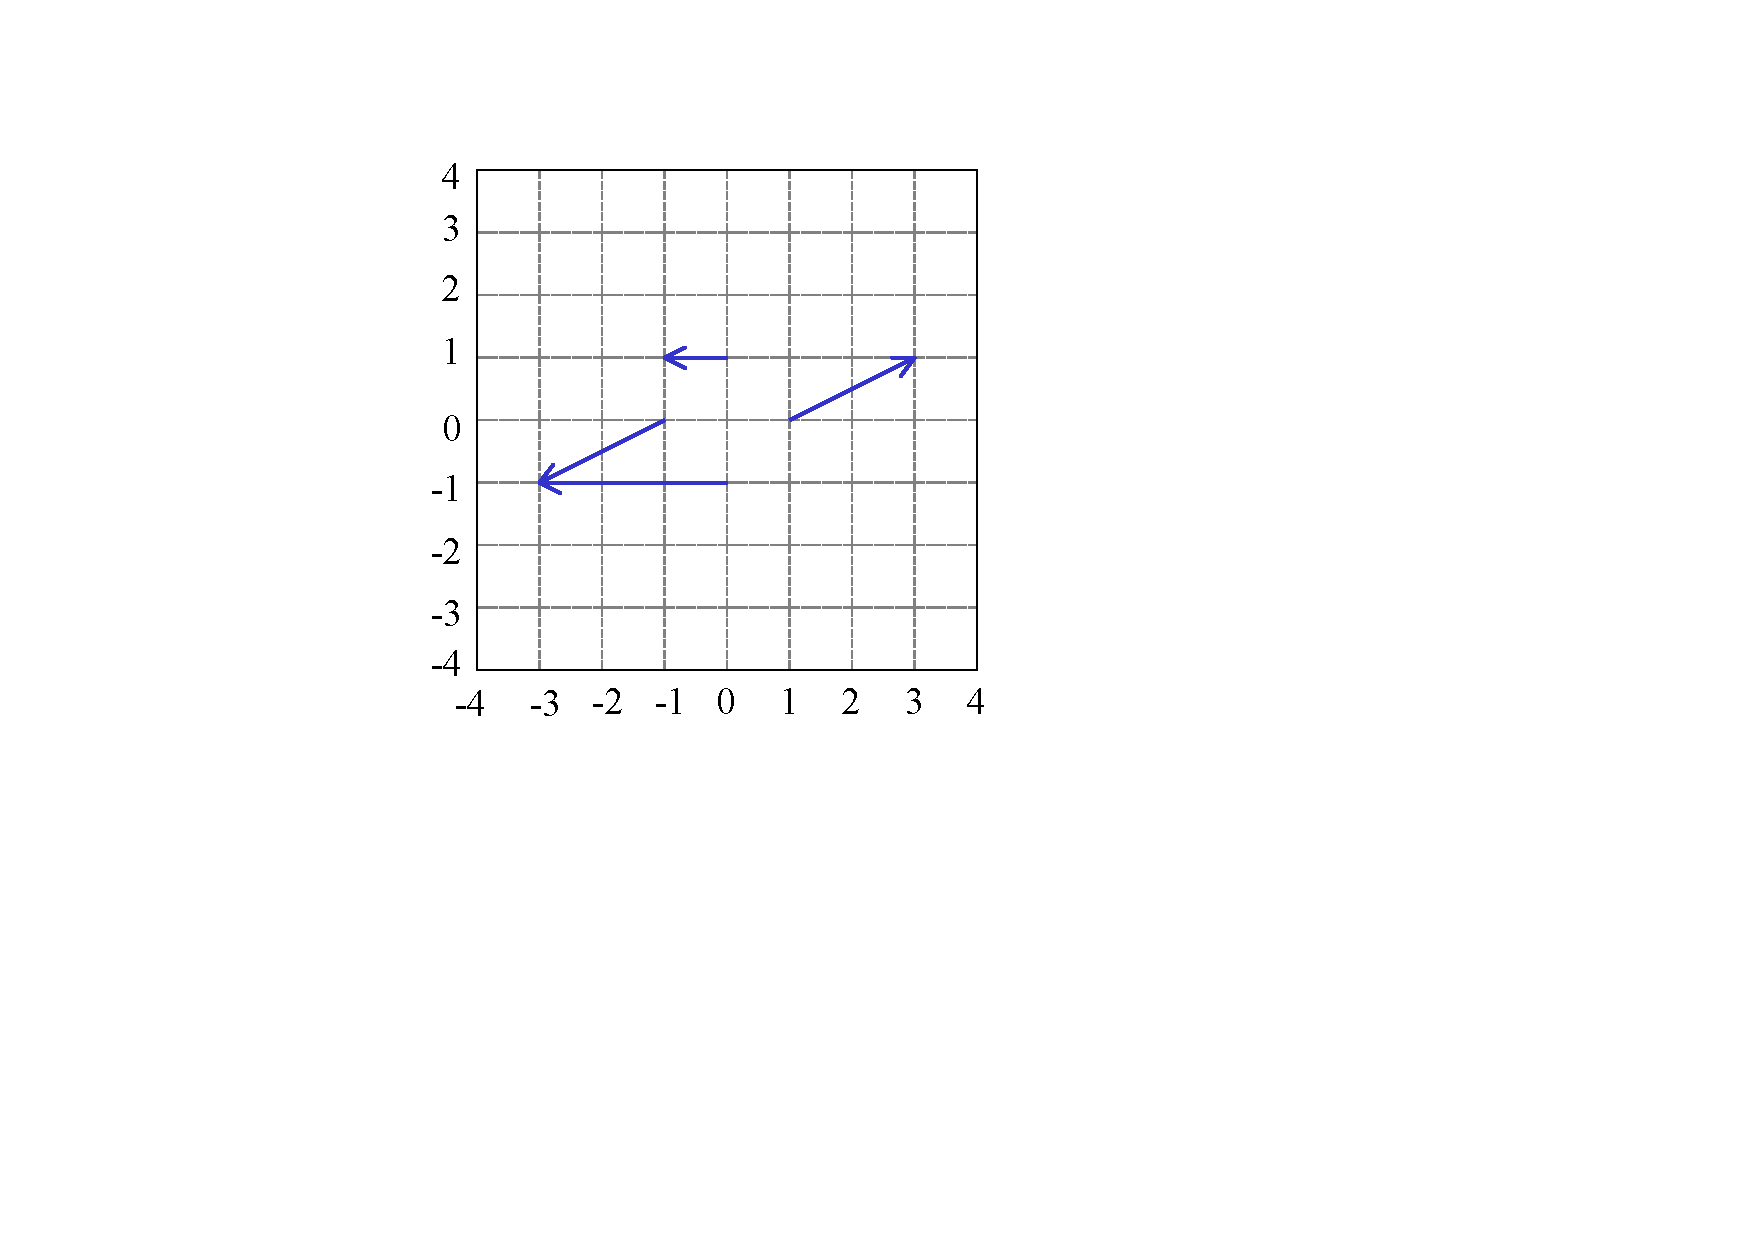
\includegraphics[scale=0.45,angle=270]{img/vectores-par-13}
\end{center}
\end{enumerate}
}
%SOLUTION
{\begin{enumerate}
\item $\nabla f(x,y) = \left(2x-2y^2+\cos(xy)y\, ,\, -4xy+\cos(xy)x\right)$  y
$\nabla g(x,y) = \left((-4x^2-6xy^2+2)\, ,\, (-4xy-6y^3+6y)\right)e^{1-x^2-y^2}$.
\item Los vectores gradientes son de la función $f$.
\end{enumerate}
}
%RESOLUTION
{\begin{enumerate}
\item Para calcular el gradiente necesitamos calcular las derivadas parciales de $f$ y $g$ con respecto a sus variables:
\begin{align*}
\frac{\partial f}{\partial x}(x,y) &= \frac{\partial}{\partial
x}\left(x^2- 2xy^2+\sen(xy)\right)=
2x-2y^2+\cos(xy)\frac{\partial}{\partial x}(xy)=2x-2y^2+\cos(xy)y,\\
\frac{\partial f}{\partial y}(x,y) &= \frac{\partial}{\partial
y}\left(x^2- 2xy^2+\sen(xy)\right)=
-4xy+\cos(xy)\frac{\partial}{\partial y}(xy)=-4xy+\cos(xy)x,\\
\frac{\partial g}{\partial x}(x,y) &= \frac{\partial}{\partial x}\left((2x+3y^2)e^{1-x^2-y^2}\right)=
\frac{\partial}{\partial x}(2x+3y^2)e^{1-x^2-y^2}+(2x+3y^2)\frac{\partial}{\partial x}e^{1-x^2-y^2}=\\
&= 2e^{1-x^2-y^2}+(2x+3y^2)e^{1-x^2-y^2}\frac{\partial}{\partial x}\left(1-x^2-y^2\right) = \\
&= 2e^{1-x^2-y^2}+(2x+3y^2)e^{1-x^2-y^2}(-2x)= (-4x^2-6xy^2+2)e^{1-x^2-y^2},\\
\frac{\partial g}{\partial y}(x,y) &= \frac{\partial}{\partial y}\left((2x+3y^2)e^{1-x^2-y^2}\right)=
\frac{\partial}{\partial x}(2x+3y^2)e^{1-x^2-y^2}+(2x+3y^2)\frac{\partial}{\partial y}e^{1-x^2-y^2}=\\
&= 6y e^{1-x^2-y^2}+(2x+3y^2)e^{1-x^2-y^2}\frac{\partial}{\partial y}\left(1-x^2-y^2\right) =\\
&=6ye^{1-x^2-y^2}+(2x+3y^2)e^{1-x^2-y^2}(-2y)= (-4xy-6y^3+6y)e^{1-x^2-y^2}.
\end{align*}
Así pues, los gradientes son
\begin{align*}
\nabla f(x,y) &=\left(\frac{\partial f}{\partial x}(x,y),\frac{\partial
f}{\partial y}(x,y)\right) = \left(2x-2y^2+\cos(xy)y\, ,\, -4xy+\cos(xy)x\right) \\
\nabla g(x,y) &=\left(\frac{\partial g}{\partial x}(x,y),\frac{\partial
g}{\partial y}(x,y)\right) = \left((-4x^2-6xy^2+2)\, ,\, (-4xy-6y^3+6y)\right)e^{1-x^2-y^2}
\end{align*}

\item Para ver a qué función corresponde la gráfica, calculamos el gradiente en los puntos que nos dan
\begin{align*}
\nabla f(1,0) &= \left(2\cdot 1-2\cdot 0^2+\cos(1\cdot 0)\cdot 0\, ,\, -4\cdot1\cdot0+\cos(1\cdot 0)\cdot1\right) =(2,1),\\
\nabla g(1,0) &= \left((-4\cdot1^2-6\cdot 1\cdot 0^2+2)\, ,\, (-4\cdot 1\cdot 0-6\cdot 0^3+6\cdot 0)\right)e^{1-1^2-0^2}= (-2,0).
\end{align*}
Como el vector libre situado en el punto $(1,0)$ es el $(2,1)$, la gráfica no puede pertenecer a la función $g(x,y)$. Para asegurarnos que se corresponde con la $f(x,y)$, calculamos el gradiente de esta función en el resto de los puntos:
\begin{align*}
\nabla f(0,1) &= \left(2\cdot 0-2\cdot 1^2+\cos(0\cdot 1)\cdot 1\, ,\, -4\cdot0\cdot1+\cos(0\cdot 1)\cdot0\right) =(-1,0),\\
\nabla f(-1,0) &= \left(2\cdot (-1)-2\cdot 0^2+\cos(-1\cdot 0)\cdot 0\, ,\, -4\cdot-1\cdot0+\cos(-1\cdot 0)\cdot(-1)\right) =(-2,-1),\\
\nabla f(0,-1) &= \left(2\cdot 0-2\cdot (-1)^2+\cos(0\cdot (-1))\cdot (-1)\, ,\, -4\cdot0\cdot(-1)+\cos(0\cdot (-1))\cdot0\right) =(-3,0).
\end{align*}
Luego los vectores de la gráfica se corresponden con los vectores gradientes de $f(x,y)$.
\end{enumerate}
}


\newproblem{par-14}{gen}{}
%STATEMENT
{Tenemos dos objetos de masas $m_1$ y $m_2$ unidas por una cuerda que pasa a través de una polea como la de la figura.
\begin{center}
  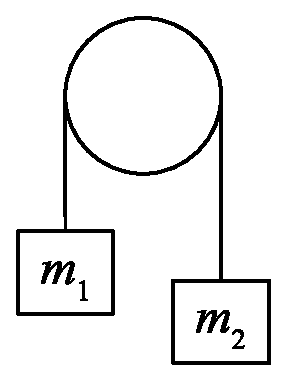
\includegraphics[scale=0.5]{img/polea-par-14}
\end{center}
Si $m_1\geq m_2$, la aceleración de $m_1$ viene dada por la ecuación
\[
a=\frac{m_1-m_2}{m_1+m_2}g,
\]
siendo $g$ la aceleración de la gravedad.
Demostrar que se cumple la ecuación
\[
m_1\frac{\partial a}{\partial m_1}+m_2\frac{\partial a}{\partial m_2}=0.
\]
}
%SOLUTION
{$\dfrac{\partial a}{\partial m_1} = \dfrac{2gm_2}{(m_1+m_2)^2}$ y $\dfrac{\partial a}{\partial m_2} = \dfrac{-2gm_1}{(m_1+m_2)^2}$.
}
%RESOLUTION
{
}


\newproblem{par-15}{gen}{*}
%STATEMENT
{The electricl potential, as a function of the distance, is given by $V=\log D$, where $D=\sqrt{x^2+y^2}$.
\begin{enumerate}
\item Compute the gradient of $V$.
\item Find the direction of biggest change of the electric potential at the point $(x,y)=(\sqrt{3},\sqrt{3})$.
\item Compute the Hessian of $V$ and its determinant at the point of part (b).
\item In which point of the curve $y=x+1$ will the potential be minimal?
\end{enumerate}
}
%SOLUTION
{\begin{enumerate}
\item $\nabla V(x,y) = \left( \frac{x}{x^2+y^2},\frac{y}{x^2+y^2}\right)$.
\item $\nabla V(\sqrt 3, \sqrt 3) = \sqrt 3 /6(1,1)$.
\item $
HV(x,y) = \left(
\begin{array}{cc}
\frac{y^2-x^2}{y^4+2x^2y^2+x^4} & \frac{-2xy}{y^4+2x^2y^2+x^4} \\
\frac{-2xy}{y^4+2x^2y^2+x^4} & \frac{x^2-y^2}{y^4+2x^2y^2+x^4}
\end{array}
\right),\quad
\left(
\begin{array}{cc}
0 & -1/6 \\
-1/6 & 0
\end{array}
\right),\quad \mbox{y }
|H(\sqrt 3,\sqrt 3)| = -1/36.
$
\item The potential is minimum at $(x=-1/2, y=1/2)$ and its value is $V(-1/2,1/2) = -\dfrac{\log 2}{2}$.
\end{enumerate}
}
%RESOLUTION
{
}


\newproblem*{par-16}{qui}{}
%STATEMENT
{La ecuación unidimensional del calor es
\[
\frac{\partial q}{\partial t}=c^2\frac{\partial^2q}{\partial x^2},
\]
donde $c$ es una constante y $q(x,t)$ es la temperatura de una varilla en un punto que ocupa la posición $x$ en el instante $t$. Demostrar que $q(x,t)=e^{ax+bt}$, con $a\neq 0$, satisface dicha ecuación para un valor apropiado de $c$.
}


\newproblem*{par-17}{amb}{*}
%STATEMENT
{Suponiendo que la temperatura, $T$ en ºC, de una zona de la atmósfera es función de la densidad del aire, $d$, en g por cm$^3$, la altura, $h$, en kilómetros, y de la concentración de un determinado elemento, $c$, en mg por cm$^3$, viene dada por la expresión:
\[
T(d,h,c) = \frac{{\ln (dh)}}{c} + c^2 3^{hd}
\]
\begin{enumerate}
\item Suponiendo que la altura a la que medimos la temperatura es de un kilómetro, y que la temperatura medida es de 0 ºC, dar la expresión de la concentración en función de la densidad.
\item Calcular el gradiente de la temperatura en el punto $(d_0,h_0,c_0)=(1,1,2)$.
\item Comprobar que se cumple que:
\[
\frac{{\partial ^2 T}}{{\partial d\partial h}} = \frac{{\partial ^2
T}}{{\partial h\partial d}}
\]
\end{enumerate}
}


\newproblem{par-18}{gen}{}
%STATEMENT
{Sea $z(x,y)=\dfrac{x^{2}}{y}+\dfrac{y^{2}}{x}.$ Calcular todas sus derivadas parciales de primer y segundo orden.
}
%SOLUTION
{$\frac{\partial z}{\partial x} = \frac{2x}{y}-\frac{y^2}{x^2}$, $\dfrac{\partial z}{\partial x} = \frac{2y}{x}-\frac{x^2}{y^2}$,\\
$\frac{\partial^2 z}{\partial x^2} = \frac{2y^2}{x^3}+\frac{2}{y}$, $\frac{\partial^2 z}{\partial y\partial x} = -\frac{2y}{x^2}-\frac{2x}{y^2}$, $\frac{\partial^2 z}{\partial x\partial y} = -\frac{2y}{x^2}-\frac{2x}{y^2}$, $\frac{\partial^2 z}{\partial x^2} = \frac{2x^2}{y^3}+\frac{2}{x}$.
}
%RESOLUTION
{
}


\newproblem*{par-19}{gen}{}
%STATEMENT
{Dada la función $f(x,y)=\dfrac{x-y}{x+y}$, hallar $\dfrac{\partial f}{\partial x}$ y $\dfrac{\partial f}{\partial y}$ en el punto $(2,-1)$.
}


\newproblem*{par-20}{amb}{*}
%STATEMENT
{Supongamos la función de varias variables $f(x,y,z)=x^{3}+\sqrt{xyz}$ que da la presión en un recipiente en función de la posición $(x,y,z)$. Suponiendo que en el recipiente hay un insecto y que se encuentra en el punto de coordenadas $(2,1,3)$, ¿en qué dirección debe moverse si busca ir lo más rápidamente posible hacia zonas de menor presión?
}


\newproblem*{par-21}{gen}{}
%STATEMENT
{Dado el siguiente campo escalar expresado en coordenadas cartesianas:
\[
f(x,y,z)=3xy\ln \left( \dfrac{1}{z}\right)
\]
Calcular:
\begin{enumerate}
\item  Su vector gradiente.
\item  Su matriz Hessiana.
\end{enumerate}
}


\newproblem*{par-22}{gen}{*}
%STATEMENT
{La definición del polinomio de Taylor de grado 2 de una función de dos variables, $f(x,y)$, centrado en el punto $(x_{0},y_{0})$, es
\begin{align*}
P_{f,(x_0,y_0)}^{2}(x,y)&= f(x_{0},y_{0})+\dfrac{\partial f(x_{0},y_{0})}{\partial x}(x-x_{0})+\dfrac{\partial f(x_{0},y_{0})}{\partial y}(y-y_{0})+\\
&+\dfrac{1}{2}\dfrac{\partial ^{2}f(x_{0},y_{0})}{\partial x^{2}}(x-x_{0})^{2}+\dfrac{1}{2}\dfrac{\partial ^{2}f(x_{0},y_{0})}{\partial y^{2}}(y-y_{0})^{2}+\dfrac{\partial ^{2}f(x_{0},y_{0})}{\partial x\partial y}(x-x_{0})(y-y_{0})
\end{align*}
\begin{enumerate}
\item  Utilizar la fórmula anterior para calcular el polinomio de Taylor de grado 2 de la función $f(x,y)=e^{(x+2y)}$ centrado en $(x_{0},y_{0})=(0,0)$.
\item  Utilizar el polinomio anterior para dar el valor aproximado de $e^{(0.1+2\cdot 0.1)}$.
\end{enumerate}
}


\newproblem*{par-23}{fis}{*}
%STATEMENT
{Suponiendo que el potencial eléctrico en un punto de coordenadas cartesianas $(x,y,z)$ viene dado por:
\[
V(x,y,z) = \frac{1} {{x{\kern 1pt} e^y \ln z}},
\]
calcular en el punto $(1,0,e)$:
\begin{enumerate}
\item El campo eléctrico (recordar que el campo eléctrico es el gradiente del potencial cambiado de signo: $\vec E =  - \vec\nabla V$).
\item La divergencia del campo eléctrico.
\end{enumerate}
}


\newproblem*{par-24}{gen}{*}
%STATEMENT
{Para la función de 2 variables $f(x,y) = x^{y^2}$
\begin{enumerate}
\item Calcular su dirección y sentido de máximo crecimiento en el punto $(1,1)$.
\item Calcular su matriz Hessiana.
\end{enumerate}
}


\newproblem{par-25}{amb}{*}
%STATEMENT
{Chemiotaxis is the movement of an organism in response to a chemical stimulus.
Usually this movement takes place in the direction in which the concentration of the checmical increases the fastest.
The Dictyoselium discoideum mold shows this type of behaviour.
The single-celled amoeba of this mold moves following the concentration of a chemical substance denoted by AMP.
Suppose the concentration of AMP at the point of coordinates $(x,y,z)$ is given by:
\[
C(x,y,z)=\frac{4}{\sqrt{x^2+y^2+z^4+1}}
\]
An amoeba is placed at the point $(-1,0,1)$, in which direction will it move?
}
%SOLUTION
{$(4/\sqrt{27}, 0, -8/\sqrt{27})$.
}
%RESOLUTION
{
}




%%%%%%% Pendiente 26




\newproblem{par-27}{qui}{*}
%STATEMENT
{Supongamos que tenemos una superficie plana, y que la cantidad de una sustancia, $C$ en g/cm$^2$,
depositada sobre cada punto de coordenadas $x$ e $y$, en metros, es función del punto y del tiempo $t$, en horas, y
viene dada por la expresión:
\[
C(x,y,t) = \sqrt{e^{-\frac{3ty}{x^2+1}}}
\]
\begin{enumerate}
\item Calcular la dirección y sentido de máximo crecimiento de la
función en el punto $(x_0,y_0,t_0)=(1,0,1)$.
\item Calcular: $\dfrac{{\partial ^2 C}}{{\partial y\partial x}}$.
\item ¿En qué puntos se anulará el gradiente de $C$?
\end{enumerate}
}
%SOLUTION
{\begin{enumerate}
\item $\nabla C(1,0,1) =\frac{1}{4}(0,-3,0)$.
\item $\displaystyle \frac{\partial^2 C}{\partial y\partial x} =
\frac{e^{-\frac{3ty}{2x^2+2}}}{(2x^2+2)^2}\left(\frac{-36t^2yx}{2x^2+2}+12tx\right)$.
\item En los puntos de la forma $(x,0,0)\ \forall x\in \mathbb{R}$.
\end{enumerate}
}
%RESOLUTION
{Antes de nada conviene simplificar la función:
\[
C(x,y,t) = \sqrt{e^{-\frac{3ty}{x^2+1}}} = \left(e^{-\frac{3ty}{x^2+1}}\right)^{1/2} = e^{-\frac{3ty}{2x^2+2}}
\]
\begin{enumerate}
\item La dirección y sentido de máximo crecimiento de una función de varias variables la da el vector gradiente, en este caso,
\[
\nabla C(x,y,t) =\left(\frac{\partial C}{\partial x}, \frac{\partial C}{\partial y}, \frac{\partial C}{\partial t} \right)
\]
Calulamos las tres derivadas parciales:
\begin{align*}
\frac{\partial C}{\partial x} &= \frac{\partial}{\partial x} e^{-\frac{3ty}{2x^2+2}} = e^{-\frac{3ty}{2x^2+2}} \frac{\partial}{\partial x}\left(-\frac{3ty}{2x^2+2}\right) = e^{-\frac{3ty}{2x^2+2}}\frac{3ty\cdot 4x}{(2x^2+2)^2} \\
\frac{\partial C}{\partial y} &= \frac{\partial}{\partial y} e^{-\frac{3ty}{2x^2+2}} = e^{-\frac{3ty}{2x^2+2}} \frac{\partial}{\partial y}\left(-\frac{3ty}{2x^2+2}\right) = e^{-\frac{3ty}{2x^2+2}}\frac{-3t}{2x^2+2} \\
\frac{\partial C}{\partial t} &= \frac{\partial}{\partial t} e^{-\frac{3ty}{2x^2+2}} = e^{-\frac{3ty}{2x^2+2}} \frac{\partial}{\partial t}\left(-\frac{3ty}{2x^2+2}\right) = e^{-\frac{3ty}{2x^2+2}}\frac{-3y}{2x^2+2}
\end{align*}
De modo que el vector gradiente es
\[
\nabla C(x,y,t) =\frac{e^{-\frac{3ty}{2x^2+2}}}{2x^2+2}\left(\frac{12tyx}{2x^2+2}, -3t, -3y\right),
\]
y en el punto $(x_0,y_0,t_0)=(1,0,1)$ vale
\[
\nabla C(1,0,1) =\frac{e^{-\frac{3\cdot 1\cdot 0}{2\cdot 1^2+2}}}{2\cdot 1^2+2}\left(\frac{12\cdot 1\cdot 0\cdot 1}{2\cdot 1^2+2}, -3\cdot 1, -3\cdot 0\right) = \frac{1}{4}(0,-3,0).
\]

\item
\begin{align*}
\frac{\partial^2 C}{\partial y\partial x} &= \frac{\partial}{\partial y}\frac{\partial C}{\partial x} e^{-\frac{3ty}{2x^2+2}} = \frac{\partial}{\partial y}  \left(e^{-\frac{3ty}{2x^2+2}}\frac{12tyx}{(2x^2+2)^2}\right) = \\
&= \frac{\partial}{\partial y} \left(e^{-\frac{3ty}{2x^2+2}}\right)\frac{12tyx}{(2x^2+2)^2}+e^{-\frac{3ty}{2x^2+2}}\frac{\partial}{\partial y}\left(\frac{12tyx}{(2x^2+2)^2}\right) = \\
&= e^{-\frac{3ty}{2x^2+2}}\frac{\partial}{\partial y}\left(-\frac{3ty}{2x^2+2}\right)\frac{3ty\cdot 4x}{(2x^2+2)^2}+e^{-\frac{3ty}{2x^2+2}}\frac{12tx}{(2x^2+2)^2} = \\
&= e^{-\frac{3ty}{2x^2+2}}\frac{-3t}{2x^2+2}\frac{3ty\cdot 4x}{(2x^2+2)^2}+e^{-\frac{3ty}{2x^2+2}}\frac{12tx}{(2x^2+2)^2} = \\
&= \frac{e^{-\frac{3ty}{2x^2+2}}}{(2x^2+2)^2}\left(\frac{-36t^2yx}{2x^2+2}+12tx\right).
\end{align*}

\item
\[
\nabla C(x,y,t) =\frac{e^{-\frac{3ty}{2x^2+2}}}{2x^2+2}\left(\frac{12tyx}{2x^2+2}, -3t, -3y\right) = (0,0,0) \Leftrightarrow
\left\{
\begin{array}{l}
12txy =0 \\
-3t = 0\\
-3y = 0
\end{array}
\right.
\]
de donde se deduce que $t=0$, $y=0$ y $x$ puede tomar cualquier valor. Así pues, los puntos que anulan el gradiente son de la forma $(x,0,0)$, $x\in\mathbb{R}$.
\end{enumerate}
}


\newproblem{par-28}{fis}{*}
%STATEMENT
{A long piece of metal is heated in such way that, at time $t$ minutes, and at $x$ meters from its left endpoint, the temperature is given by
$H(x,t) = 100e^{-0.1t}\sin(\pi xt)$ with $0\leq x \leq 1$.
\begin{enumerate}
\item Compute $\dfrac{\partial H}{\partial x}(0.2, 1)$ and $\dfrac{\partial H}{\partial x}(0.8, 1)$.
What is the meaning (in terms of the temperature) of these two partial derivatives? Explain the sign of each partial derivative.
\item Compute the Hessian of $H$.
\end{enumerate}
}
%SOLUTION
{\begin{enumerate}
\item $\frac{\partial H}{\partial x}(0.2,\, 1) = 100e^{-0.1}\cos(0.2\pi) \pi = 229.9736$ \\
$\frac{\partial H}{\partial x}(0.8,\, 1) = 100e^{-0.1}\cos(0.8\pi) \pi = -229.9736$.
\item \resizebox{\linewidth}{!}{$
\left(
\begin{array}{cc}
-100e^{-0.1t}\pi^2 t^2\sen(\pi xt) & 100e^{-0.1t}\left((-0.1\pi t+\pi)\cos(\pi xt) - \pi^2 xt \sen(\pi xt)\right) \\
100e^{-0.1t}\left((-0.1\pi t+\pi)\cos(\pi xt) - \pi^2 xt \sen(\pi xt)\right) & 100e^{-0.1t}\left(0.01\sen(\pi xt) -(0.2+\pi^2x^2) \cos(\pi xt)\right)
\end{array}
\right)$}
\end{enumerate}
}
%RESOLUTION
{\begin{enumerate}
\item La derivada parcial de $H$ con respecto a $x$ es
\begin{align*}
\frac{\partial H}{\partial x}(x,t) &= 100e^{-0.1t}\cos(\pi xt) \pi t \\
\end{align*}
y en los puntos que nos piden vale
\begin{align*}
\frac{\partial H}{\partial x}(0.2,\, 1) &= 100e^{-0.1}\cos(0.2\pi) \pi =
229.9736\\
\frac{\partial H}{\partial x}(0.8,\, 1) &= 100e^{-0.1}\cos(0.8\pi) \pi =
-229.9736
\end{align*}
La derivada parcial $\dfrac{\partial H}{\partial x}(x_0,t_0)$ indica la variación instantánea que experimenta la temperatura con respecto a la variación de la distancia al extremo izquierdo en el punto. El signo de la derviada parcial indica si la variación de la temperatura es creciente (aumenta la temperatura) o decreciente (disminuye). Así en el punto $(0.2,\, 1)$ la temperatura aumentará a razón de $229.9736$ grados centígrados por cada metro que nos alejemos del extremo izquierdo de la barra de metal, mientras que en el $(0.8,\,1)$ la temperatura disminuirá a razón de $229.9736$ grados centígrados por cada metro que nos alejemos del extremo izquierdo de la barra de metal.

\item Para calcular la matriz Hessiana necesitamos las derivadas parciales de
segundo orden:
\begin{align*}
\frac{\partial H}{\partial t} (x,t) &= 100\left(\frac{\partial}{\partial x} e^{-0.1 t} \sen (\pi xt) + e^{-0.1t}\frac{\partial}{\partial x}\sen(\pi xt)\right)=\\
&= 100\left(-0.1e^{-0.1t}\sen(\pi xt) +e^{-0.1t}\cos(\pi xt)\pi x\right) =\\
&= 100 e^{-0.1t}\left(-0.1 \sen(\pi xt) + \pi x \cos(\pi xt)\right),\\
\frac{\partial^2 H}{\partial x^2}(x,t) &= \frac{\partial}{\partial x}\left(100e^{-0.1t}\pi t\cos(\pi xt) \right) = 100e^{-0.1t}\pi t(-\sen(\pi xt) \pi t) =\\
&= -100e^{-0.1t}\pi^2 t^2\sen(\pi xt),\\
\frac{\partial^2 H}{\partial t\partial x}(x,t) &= \frac{\partial}{\partial t}\left(100e^{-0.1t}\pi t\cos(\pi xt) \right) =\\
&= 100\left(\frac{\partial}{\partial t}e^{-0.1t}\pi t\cos(\pi xt) + e^{-0.1t}\left(\frac{\partial}{\partial t}(\pi t)\cos(\pi xt) + \pi t \frac{\partial}{\partial t}\cos(\pi xt)\right) \right) =\\
&= 100\left(-0.1e^{-0.1t}\pi t\cos(\pi xt) + e^{-0.1t}\left(\pi \cos(\pi xt) - \pi t \sen(\pi xt)\pi x\right) \right) =\\
&= 100e^{-0.1t}\left(-0.1\pi t\cos(\pi xt)+\pi \cos(\pi xt) - \pi^2 xt \sen(\pi xt)\right) = \\
&= 100e^{-0.1t}\left((-0.1\pi t+\pi)\cos(\pi xt) - \pi^2 xt \sen(\pi xt)\right),\\
\end{align*}

\begin{align*}
\frac{\partial^2 H}{\partial x\partial t}(x,t) &= \frac{\partial^2 H}{\partial t\partial x}(x,t) \quad (\mbox{igualdad de las derivadas cruzadas por el teorema de Schwartz})\\
\frac{\partial^2 H}{\partial t^2}(x,t) &= \frac{\partial}{\partial t} \left(100 e^{-0.1t}\left(-0.1 \sen(\pi xt) + \pi x \cos(\pi xt)\right)\right)  =\\
&= 100\left(\frac{\partial}{\partial t} e^{-0.1t}\left(-0.1 \sen(\pi xt) + \pi x \cos(\pi xt)\right) +\right.\\
&\left. \qquad + e^{0.1t}\left(\frac{\partial}{\partial t}\left(-0.1\sen(\pi xt)\right) + \frac{\partial}{\partial t}\left(\pi x \cos(\pi xt)\right)\right)\right) =\\
&= 100\left(-0.1 e^{-0.1t}\left(-0.1 \sen(\pi xt) + \pi x \cos(\pi xt)\right)\right. +\\
&\left. \qquad + e^{0.1t}\left(-0.1\cos(\pi xt)\pi x - \pi x \cos(\pi xt)\pi x\right)\right) =\\
&= 100e^{-0.1t}\left(0.01\sen(\pi xt) -0.1 \pi x \cos(\pi xt) -0.1\pi x\cos(\pi xt) - \pi^2 x^2 \cos(\pi xt)\right) = \\
&= 100e^{-0.1t}\left(0.01\sen(\pi xt) -(0.2+\pi^2x^2) \cos(\pi xt)\right).
\end{align*}
Así pues, la matriz Hessiana es
\[
\left(
\begin{array}{cc}
-100e^{-0.1t}\pi^2 t^2\sen(\pi xt) & 100e^{-0.1t}\left((-0.1\pi t+\pi)\cos(\pi xt) - \pi^2 xt \sen(\pi xt)\right) \\
100e^{-0.1t}\left((-0.1\pi t+\pi)\cos(\pi xt) - \pi^2 xt \sen(\pi xt)\right) & 100e^{-0.1t}\left(0.01\sen(\pi xt) -(0.2+\pi^2x^2) \cos(\pi xt)\right)
\end{array}
\right)
\]
\end{enumerate}
}


\newproblem{par-29}{gen}{*}
%STATEMENT
{Dar la dirección de máximo crecimiento de la función
\[
f(x,y,z) = \frac{\log(zx)}z-xe^{-zxy}
\]
en el punto $(1,1,1)$.
}
%SOLUTION
{$\nabla f(1,1,1)=(1,e^{-1},1+e^{-1})$.
}
%RESOLUTION
{La dirección de máximo crecimiento de una función de varias variables la da el vector gradiente:
\[
\nabla f(x,y,z) = \left(\frac{\partial f}{\partial x}(x,y,z),\frac{\partial f}{\partial y}(x,y,z),\frac{\partial f}{\partial z}(x,y,z)\right)
\]
Calculamos por tanto cada una de las derivadas parciales que aparecen en las componentes del vector:
\begin{align*}
\frac{\partial f}{\partial x}(x,y,z) &= \frac{\partial}{\partial x}(\frac{\log (zx)}z-xe^{-zxy}) = \frac{\partial}{\partial x}(\frac{\log (zx)}z)-\frac{\partial}{\partial x}(xe^{-zxy})= \\
&= \frac{1}{z}\frac{\partial}{\partial x}(\log (zx))-(\frac{\partial}{\partial x}(x)e^{-zxy}+x\frac{\partial}{\partial x}(e^{-zxy}))= \\
&= \frac{1}{z}\frac{1}{zx}\frac{\partial}{\partial x}(zx)-(e^{-zxy}+xe^{-zxy}\frac{\partial}{\partial x}(-zxy))= \\
&= \frac{1}{z}\frac{1}{zx}z-(e^{-zxy}+xe^{-zxy}(-zy)) = \frac{1}{zx}-e^{-zxy}(1-xyz),\\
\frac{\partial f}{\partial y}(x,y,z) &= \frac{\partial}{\partial y}(\frac{\log(zx)}z-xe^{-zxy}) = \frac{\partial}{\partial y}(\frac{\log (zx)}z)-\frac{\partial}{\partial y}(xe^{-zxy})= \\
&= -x\frac{\partial}{\partial y}(e^{-zxy}) = -xe^{-zxy}\frac{\partial}{\partial y}(-zxy)=x^2ze^{-zxy},\\
\frac{\partial f}{\partial z}(x,y,z) &= \frac{\partial}{\partial z}(\frac{\log(zx)}z-xe^{-zxy}) = \frac{\partial}{\partial z}(\frac{\log (zx)}z)-\frac{\partial}{\partial z}(xe^{-zxy})= \\
&= \frac{\frac{\partial}{\partial z}(\log (zx))z-\log (zx)\frac{\partial}{\partial z}(z)}{z^2}-x\frac{\partial}{\partial z}(e^{-zxy}))= \\
&= \frac{\frac 1{zx}\frac \partial {\partial z}(zx)z-\log (zx)}{z^2}-xe^{-zxy}\frac{\partial}{\partial z}(-zxy))= \\
&= \frac{\frac 1{zx}xz-\log (zx)}{z^2}-xe^{-zxy}-xy=\frac{1-\log (zx)}{z^2}+x^2ye^{-zxy}.
\end{align*}
Por lo tanto, el vector gradiente será:
\[
\nabla f(x,y,z)=(\frac{1}{zx}-e^{-zxy}(1-xyz), x^2ze^{-zxy}, \frac{1-\log (zx)}{z^2}+x^2ye^{-zxy})
\]

Finalmente, como nos pieden la dirección de máximo crecimiento en el punto $(1,1,1)$, tendremos que particularizar el vector gradiente en dicho punto, es decir:
\[
\nabla f(1,1,1)=(1,e^{-1},1+e^{-1}).
\]
}


\newproblem{par-30}{gen}{*}
%STATEMENT
{Calcular el gradiente de la función
\[
f(x,y,z)=e^{\sqrt{x^2+2yz}}+\ln (\frac{xy}z)
\]
en el punto $(1,-2,-2)$.
}
%SOLUTION
{$\nabla f(x,y,z)=\left(\frac{xe^{\sqrt{x^2+2yz}}}{\sqrt{x^2+2yz}}+\frac{1}{x}, \frac{ze^{\sqrt{x^2+2yz}}}{\sqrt{x^2+2yz}}+\frac{1}{y}, \frac{ye^{\sqrt{x^2+2yz}}}{\sqrt{x^2+2yz}}-\frac{1}{z}\right)$\\ y $\nabla f(1,-2,-2)=\left(\frac{e^3}{3}+1,\frac{-2e^3}{3}-\frac{1}{2},\frac{-2e^3}{3}+\frac{1}{2}\right)$.}
%RESOLUTION
{El gradiente de $f(x,y,z)$ se define como el vector $\nabla f(x,y,z)=\left(\dfrac{\partial f}{\partial x}(x,y,z),\dfrac{\partial f}{\partial y}(x,y,z),\dfrac{\partial f}{\partial z}(x,y,z)\right).$ Por tanto, tenemos que calcular las tres derivadas parciales siguientes:
\begin{align*}
\dfrac{\partial f}{\partial x}(x,y,z) &= \dfrac{\partial}{\partial x}(e^{\sqrt{x^2+2yz}}+\ln (\frac{xy}z)) = \dfrac{\partial}{\partial x}(e^{\sqrt{x^2+2yz}})+\dfrac{\partial}{\partial x}(\ln (\frac{xy}z))= \\
&= e^{\sqrt{x^2+2yz}}\dfrac \partial {\partial x}(\sqrt{x^2+2yz})+\frac{1}{xy/z}\dfrac{\partial}{\partial x}(\frac{xy}z)= \\
&= e^{\sqrt{x^2+2yz}}\frac{1}{2\sqrt{x^2+2yz}}\dfrac{\partial}{\partial x}(x^2+2yz)+\frac{z}{xy}\frac{y}{z}= \\
&= e^{\sqrt{x^2+2yz}}\frac{1}{2\sqrt{x^2+2yz}}2x+\frac{1}{x} = \frac{xe^{\sqrt{x^2+2yz}}}{\sqrt{x^2+2yz}}+\frac{1}{x}, \\
\dfrac{\partial f}{\partial y}(x,y,z) &= \dfrac{\partial}{\partial y}(e^{\sqrt{x^2+2yz}}+\ln (\frac{xy}z)) = \dfrac{\partial}{\partial y}(e^{\sqrt{x^2+2yz}})+\dfrac{\partial}{\partial y}(\ln (\frac{xy}z))= \\
&= e^{\sqrt{x^2+2yz}}\dfrac{\partial}{\partial y}(\sqrt{x^2+2yz})+\frac{1}{xy/z}\dfrac{\partial}{\partial y}(\frac{xy}z)= \\
&= e^{\sqrt{x^2+2yz}}\frac{1}{2\sqrt{x^2+2yz}}\dfrac{\partial}{\partial y}(x^2+2yz)+\frac{z}{xy}\frac{x}{z}= \\
&= e^{\sqrt{x^2+2yz}}\frac{1}{2\sqrt{x^2+2yz}}2z+\frac{1}{y}=\frac{ze^{\sqrt{x^2+2yz}}}{\sqrt{x^2+2yz}}+\frac{1}{y}, \\
\dfrac{\partial f}{\partial z}(x,y,z) &= \dfrac{\partial}{\partial z}(e^{\sqrt{x^2+2yz}}+\ln (\frac{xy}z)) = \dfrac{\partial}{\partial z}(e^{\sqrt{x^2+2yz}})+\dfrac{\partial}{\partial z}(\ln (\frac{xy}{z}))= \\
&= e^{\sqrt{x^2+2yz}}\dfrac{\partial}{\partial z}(\sqrt{x^2+2yz})+\frac{1}{xy/z}\dfrac{\partial}{\partial z}(\frac{xy}{z})= \\
&= e^{\sqrt{x^2+2yz}}\frac{1}{2\sqrt{x^2+2yz}}\dfrac{\partial}{\partial z}(x^2+2yz)+\frac{z}{xy}\frac{-xy}{z^2}= \\
&= e^{\sqrt{x^2+2yz}}\frac{1}{2\sqrt{x^2+2yz}}2y-\frac{1}{z} = \frac{ye^{\sqrt{x^2+2yz}}}{\sqrt{x^2+2yz}}-\frac{1}{z},
\end{align*}
y, en consecuencia tenemos
\[
\nabla f(x,y,z)=\left(\frac{xe^{\sqrt{x^2+2yz}}}{\sqrt{x^2+2yz}}+\frac{1}{x}, \frac{ze^{\sqrt{x^2+2yz}}}{\sqrt{x^2+2yz}}+\frac{1}{y}, \frac{ye^{\sqrt{x^2+2yz}}}{\sqrt{x^2+2yz}}-\frac{1}{z}\right).
\]
Como nos piden el gradiente en el punto $(1,-2,-2),$ sustituimos $x$ por 1, $y$ por -2, y $z$ por -2 en el vector anterior y obtenemos
\[
\nabla f(1,-2,-2)=\left(\frac{e^3}{3}+1,\frac{-2e^3}{3}-\frac{1}{2},\frac{-2e^3}{3}+\frac{1}{2}\right).
\]
}


\newproblem{par-31}{gen}{*}
%STATEMENT
{Calcular el vector gradiente de la función
\[
\log \left( \sqrt{x^{2}-z^{2}}\right) +3^{\tfrac{x^{2}}{y}}
\]
en el punto $(1,1,0)$.
}
%SOLUTION
{$\nabla f(x,y,z)=(\frac{x}{x^{2}-z^{2}}+3^{\tfrac{x^{2}}{y}}\log 3\dfrac{2x}{y},3^{\tfrac{x^{2}}{y}}\log 3\dfrac{-x^{2}}{y^{2}},-\frac{z}{x^{2}-z^{2}})$, y $\nabla f(1,-2,-2)=(1+6\log 3,-3\log 3,0)$.
}
%RESOLUTION
{El gradiente de $f(x,y,z)$ se define como el vector $\nabla f(x,y,z)=(\dfrac{\partial f}{\partial x}(x,y,z),\dfrac{\partial f}{\partial y}(x,y,z),\dfrac{\partial f}{\partial z}(x,y,z))$. Por tanto, tenemos que calcular las tres derivadas parciales siguientes:
\begin{align*}
\dfrac{\partial f}{\partial x}(x,y,z) &= \dfrac{\partial }{\partial x}(\log\left(\sqrt{x^{2}-z^{2}}\right) +3^{\tfrac{x^{2}}{y}}) = \dfrac{\partial }{\partial x}(\log \left(\sqrt{x^{2}-z^{2}}\right) )+\dfrac{\partial }{\partial x}(3^{\tfrac{x^{2}}{y}})= \\
&= \frac{1}{\sqrt{x^{2}-z^{2}}}\dfrac{\partial }{\partial x}(\sqrt{x^{2}-z^{2}})+3^{\tfrac{x^{2}}{y}}\log 3\dfrac{\partial }{\partial x}(\dfrac{x^{2}}{y}) = \\
&= \frac{1}{\sqrt{x^{2}-z^{2}}}\frac{1}{2\sqrt{x^{2}-z^{2}}}\dfrac{\partial}{\partial x}(x^{2}-z^{2})+3^{\tfrac{x^{2}}{y}}\log 3\dfrac{2x}{y}= \\
&= \frac{1}{2(x^{2}-z^{2})}2x+3^{\tfrac{x^{2}}{y}}\log 3\dfrac{2x}{y}=\frac{x}{x^{2}-z^{2}}+3^{\tfrac{x^{2}}{y}}\log 3\dfrac{2x}{y}, \\
\dfrac{\partial f}{\partial y}(x,y,z) &= \dfrac{\partial }{\partial y}(\log\left( \sqrt{x^{2}-z^{2}}\right) +3^{\tfrac{x^{2}}{y}}) = \dfrac{\partial }{\partial y}(\log \left( \sqrt{x^{2}-z^{2}}\right) )+\dfrac{\partial }{\partial y}(3^{\tfrac{x^{2}}{y}})= \\
&= 0+3^{\tfrac{x^{2}}{y}}\log 3\dfrac{\partial }{\partial y}(\dfrac{x^{2}}{y}) = 3^{\tfrac{x^{2}}{y}}\log 3\dfrac{-x^{2}}{y^{2}}, \\
\dfrac{\partial f}{\partial z}(x,y,z) &= \dfrac{\partial }{\partial z}(\log\left( \sqrt{x^{2}-z^{2}}\right) +3^{\tfrac{x^{2}}{y}}) = \dfrac{\partial }{\partial z}(\log \left( \sqrt{x^{2}-z^{2}}\right) )+\dfrac{\partial }{\partial z}(3^{\tfrac{x^{2}}{y}})= \\
&= \frac{1}{\sqrt{x^{2}-z^{2}}}\dfrac{\partial }{\partial x}(\sqrt{x^{2}-z^{2}})+0 = \frac{1}{\sqrt{x^{2}-z^{2}}}\frac{1}{2\sqrt{x^{2}-z^{2}}}\dfrac{\partial }{\partial x}(x^{2}-z^{2})= \\
&= \frac{1}{2(x^{2}-z^{2})}(-2z)=-\frac{z}{x^{2}-z^{2}}.
\end{align*}
y, en consecuencia tenemos
\[
\nabla f(x,y,z)=(\frac{x}{x^{2}-z^{2}}+3^{\tfrac{x^{2}}{y}}\log 3\dfrac{2x}{y},3^{\tfrac{x^{2}}{y}}\log 3\dfrac{-x^{2}}{y^{2}},-\frac{z}{x^{2}-z^{2}}).
\]
Como nos piden el gradiente en el punto $(1,1,0),$ sustituimos $x$ por 1, $y$
por 1, y $z$ por 0 en el vector anterior y obtenemos
\[
\nabla f(1,-2,-2)=(1+6\log 3,-3\log 3,0).
\]
}


\newproblem{par-32}{amb}{}
%STATEMENT
{The amount of CO$_2$ absorbed by a plant depends on the ambient temperature ($t$) and the intensity of light ($l$), according to the following
function, where $c$ is a constant:
\[
f(t,l) = ctl^2,
\]
Study the change on the absortion of CO$_2$ for different values of the intensity of light, assuming the temperature is constant.
Do the reverse study; that is, keeing light constant, study the absortion depending on different values of the temperature.
}
%SOLUTION
{$\frac{\partial f}{\partial l}(t,l) = 2ctl$ and $\frac{\partial f}{\partial t}(t,l) = cl^2$.
}
%RESOLUTION
{
}


\newproblem{par-33}{amb}{}
%STATEMENT
{The number of plants of certain species on a field depends on the level of nitrogen on the ground, and the level of movement on the field.
An increment on nitrogen, or on movement, results on a negative effect for the plant.
Suppose that at certain point on time the level of nitrogen increases, and there is an increase on the amount of movement
due to the presence of cattle; how do these two factors affect the change in the number of plants in the field?
}
%SOLUTION
{The number of plants will decrease.
}
%RESOLUTION
{
}


\newproblem{par-34}{amb}{}
%STATEMENT
{The speed at which certain organism grows is a function of the amount of available food and the number of other organisms fighting for
food.
How will this speed change when the food available increases in quantity, and competitors decrease in number?
}
%SOLUTION
{The growth speed will increase.
}
%RESOLUTION
{
}


\newproblem{par-35}{amb}{}
%STATEMENT
{A bug moving on a surface follows always the direction of steepest descent.
If the equation of the surface is given by
\[
f(x,y)=x^2-y^2,
\]
find the direction the bug will follow from the point $(2,3)$.
}
%SOLUTION
{It will follow the direcction $-\nabla f(2,3)=(-4,6)$.}
%RESOLUTION
{
}


\newproblem{par-36}{gen}{}
%STATEMENT
{Compute $(f\circ g)'(t)$, assuming $f(x,y,z)=x^3y^2z$ and $g(t)=(e^t,\cos t,\sin t)$.
}
%SOLUTION
{$(f\circ g)'(t)= e^{3t}(3\sen t\cos^2 t-2\sen^2 t\cos t+\cos^3 t)$.
}
%RESOLUTION
{
}


\newproblem{par-37}{amb}{}
%STATEMENT
{Find the critical points of $z=f(x,y)$ in the following cases:
\begin{enumerate}
\item $f(x,y)=x^2+y^2$.
\item $f(x,y)=x^2y+y^2x$.
\item $f(x,y)=x^2-2xy+2y^2$.
\end{enumerate}
}
%SOLUTION
{\begin{enumerate}
\item $(0,0)$.
\item $(0,0)$.
\item $(0,0)$.
\end{enumerate}
}
%RESOLUTION
{
}


\newproblem{par-38}{gen}{}
%STATEMENT
{The surface of a mountain peak is given by the equation displayed below, where $a$, $b$ and $c$ are constants; and $x$ and $y$ are the East-West
and North-South coordinates, respectively.
\[
S:z=a-bx^2-cy^2,
\]
Find the direction of steepest increase of the height of the mountain if we are located at the point $P=(1,1)$.
}
%SOLUTION
{$(-2b,-2c)$.
}
%RESOLUTION
{
}


\newproblem{par-39}{gen}{}
%STATEMENT
{Find the directions of maximum increase and decrease of the following functions, at the given point $P$:
\begin{enumerate}
\item $f(x,y)=x^2+xy+y^2$, $P=(-1,1)$.
\item $f(x,y)=x^2y+e^{xy}\sin y$, $P=(1,0)$.
\item $f(x,y,z)=\log(xy)+\log(yz)+\log(xz)$, $P=(1,1,1)$.
\item $f(x,y,z)=\log(x^2+y^2-1)+y+6z$, $P=(1,1,0)$.
\end{enumerate}
}
%SOLUTION
{\begin{enumerate}
\item Maximun increase in direction $(-1,1)$ and maximum decrease in direction $(1,-1)$.
\item Maximun increase in direction $(0,2)$ and maximum decrease in direction $(0,-2)$.
\item Maximun increase in direction$(2,2,2)$ and maximum decrease in direction $(-2,-2,-2)$.
\item Maximun increase in direction $(2,3,6)$ and maximum decrease in direction $(-2,-3,-6)$.
\end{enumerate}
}
%RESOLUTION
{
}


\newproblem{par-40}{gen}{}
%STATEMENT
{Find for which directions the directional derivative of the function $f$ below at the point $P=(1,1)$ vanishes?
\[
f(x,y)=\frac{x^2-y^2}{x^2+y^2}
\]
}
%SOLUTION
{Direction $(1/\sqrt{2},1/\sqrt{2})$.
}
%RESOLUTION
{
}


\newproblem{par-41}{gen}{}
%STATEMENT
{Does there exist a direction on which the directional derivative
of the function $f$ below takes the value $14$ at the point $P=(1,2)$?
\[
f(x,y) = x^2-3xy+4y^2
\]
}
%SOLUTION
{No.
}
%RESOLUTION
{
}


\newproblem{par-42}{gen}{}
%STATEMENT
{The maximum value of the directional derivative of a function $f$ at the point $P$ is equal to $2\sqrt{3}$, and it takes place in the
direction of the vector $(1,1,-1)$.
Compute the value of the directional derivative of $f$ at $P$ in the direction $(1,1,0)$?
}
%SOLUTION
{$2\sqrt{2}$.
}
%RESOLUTION
{
}


\newproblem{par-43}{gen}{}
%STATEMENT
{Given the scalar field
\[
f(x,y,z) = x^2-y^2+xyz^3-zx
\]
and the point $P=(1,2,3)$, compute the following:
\begin{enumerate}
\item The directional derivative of $f$ at $P$ in the direction of the unit vector $\mathbf{u}=\frac{1}{\sqrt2}(1,-1,0)$.
\item The direction for which the directional derivative of $f$ at $P$ takes its maximum value.
Find such value.
\end{enumerate}
}
%SOLUTION
{\begin{enumerate}
\item $15\sqrt{2}$.
\item The directional derivative takes its maximum value in direction $(53,23,53)$ and its value is $\sqrt{6147}$.
\end{enumerate}
}
%RESOLUTION
{
}


\newproblem*{par-44}{gen}{}
%STATEMENT
{En el ajuste de regresión de una recta $y=a+bx$, se suele utilizar la técnica de mínimos cuadrados que consisten en buscar los valores
de $a$ y $b$ que hacen mínima la función
\[
f(a,b)= \sum_{i=1}^{n}(y_i-a-bx_i)^2,
\]
donde el sumatorio abarca a todos los pares de la muestra $(x_i,y_i)$ para $i=1,\ldots, n$, siendo $n$ el tamaño de la muestra.

Demostrar que esta función alcanza el mínimo en los puntos
\[
a=\bar y-b\bar x \quad \mbox{ y } b=\frac{s_{xy}}{s_x^2}.
\]
}
%SOLUTION
{
}
%RESOLUTION
{
}


\newproblem{par-45}{gen}{*}
%STATEMENT
{The function below measures the air pressure at position $(x,y,z)$.
\[
f(x,y,z)= x^2+y^2-z^3
\]
Consider an object $A$ moving along the following trajectory:
\[
\begin{cases}
x=t\\
y=1\\
z=1/t
\end{cases}
t>0.
\]
\begin{enumerate}
\item Give an equation of the tangent line to the trajectory of $A$ at
the point $(1,1,1)$.
\item Is the trajectory of $A$ at the point $(1,1,1)$ moving in the
direction of maximum increase of the function $f$?
\end{enumerate}
}
%SOLUTION
{
\begin{enumerate}
\item $(1+t, 1, 1-t)$.
\item No, as the direction of maximum increase of $f$ is $\nabla f(1,1,1)=(2,2,-3)$ and the direccion of the trajectory is $(1,0,-1)$.
\end{enumerate}
}
%RESOLUTION
{
}


\newproblem{par-46}{gen}{*}
%STATEMENT
{Compute the equation of the tangent plane and the normal line to the surface
\[
S:xyz=8
\]
at point $P=(4,-2,-1)$.
}
%SOLUTION
{Normal line $l:(4+2t,-2-4t,-1-8t)$. Tangent plane $\pi: 2x-4y-8z+24=0$.
}
%RESOLUTION
{
}



%%%%%%% Pendiente 26
